\documentclass[12pt]{article}
\usepackage{sbc-template}
\usepackage{graphicx,url}
\IfFileExists{brazil.ldf}{\usepackage[brazil]{babel}}{\usepackage[english]{babel}\addto\captionsenglish{\renewcommand{\figurename}{Figura}\renewcommand{\tablename}{Tabela}\renewcommand{\refname}{Refer\^encias}}\hyphenpenalty=10000\exhyphenpenalty=10000}
\usepackage[utf8]{inputenc}
\usepackage[T1]{fontenc}
\usepackage{amsmath,amssymb}
\usepackage{booktabs}
\usepackage{array}
\newcolumntype{L}[1]{>{\raggedright\arraybackslash}p{#1}}
\sloppy


\title{Etapa 1 -- Modelagem e Planejamento\\ Roteamento e Carga de Veículos em Centros Logísticos}

\author{João Gabriel Maia da Costa\inst{1}, Thomas Ramos Oliveira\inst{1},\\ Pedro Eduardo Pimenta\inst{1}}

\address{Engenharia de Software -- Pontifícia Universidade Católica de Minas Gerais (PUC Minas)\\ Teoria dos Grafos -- Trabalho Prático, Tema 10}

\begin{document}
\maketitle

\begin{abstract}
This document presents the first stage of a graph-based tool for planning logistics routes under capacity, time-window, distance and priority constraints. It defines the problem, justifies the graph model, selects the algorithms, specifies the architecture with UML diagrams and lays out the development plan.
\end{abstract}

\begin{resumo}
Este documento apresenta a primeira etapa de uma ferramenta, baseada em grafos, para planejar rotas logísticas com restrições de capacidade, janelas de tempo, distância e prioridade. Ele define o problema, justifica a modelagem em grafos, seleciona os algoritmos, especifica a arquitetura com diagramas UML e apresenta o plano de desenvolvimento.
\end{resumo}

\section{Contextualização e escopo}

Um centro logístico recebe pedidos de clientes espalhados em uma região e precisa decidir quais veículos saem do depósito, quais clientes cada um atende e em que ordem. A decisão afeta custo de combustível, número de veículos usados, cumprimento de horários combinados com os clientes e atendimento de pedidos urgentes. Esse é o problema clássico de roteamento de veículos~\cite{dantzig1959,tothvigo2014}.

O tema escolhido é o \textbf{Tema 10}: \emph{roteamento e carga de veículos em centros logísticos, com restrições de tempo, distância, prioridade e capacidade de carga dos veículos}. O trabalho se limita a esse tema. Ficam fora do escopo frota heterogênea, vários depósitos, coleta e entrega simultâneas e demandas estocásticas. O grafo é a base de tudo: os custos vêm dele, os algoritmos percorrem seus arcos e a verificação confere se cada trecho de rota existe nele.

\section{Definição do problema}

\subsection{Dados de entrada}

Há um depósito (vértice $0$) e um conjunto $C=\{1,\dots,n\}$ de clientes. Cada cliente $i$ tem demanda $q_i$, janela de tempo $[e_i,l_i]$, tempo de serviço $\sigma_i$ e prioridade $p_i\in\{1,2,3\}$ (alta, média, baixa). O depósito tem janela $[e_0,l_0]$. Os veículos são idênticos, com capacidade $Q$, no máximo $K$ disponíveis e, opcionalmente, distância máxima $D_{\max}$ por rota. Todos os dados do problema são conhecidos antes de planejar, e cada cliente é atendido por exatamente um veículo, em uma única visita.

\subsection{Rotas viáveis}

Uma rota $r=(0,i_1,\dots,i_m,0)$ é viável quando atende às quatro restrições do tema:
\begin{itemize}
  \item \textbf{Capacidade:} $\sum_{k} q_{i_k}\le Q$.
  \item \textbf{Tempo:} com $s_{i_1}=\max(e_{i_1},e_0+t_{0,i_1})$ e $s_{i_k}=\max(e_{i_k},\,s_{i_{k-1}}+\sigma_{i_{k-1}}+t_{i_{k-1},i_k})$, vale $s_{i_k}\le l_{i_k}$ para todo $k$ e o retorno ao depósito ocorre até $l_0$. Chegar antes de $e_i$ obriga o veículo a esperar.
  \item \textbf{Distância:} $d(r)=\sum_k d_{i_{k-1},i_k}\le D_{\max}$, quando houver limite.
  \item \textbf{Prioridade:} tratada no objetivo (a seguir), para que clientes urgentes sejam atendidos mais cedo sem tornar o problema inviável.
\end{itemize}

\subsection{Objetivo}

Encontrar um conjunto de no máximo $K$ rotas viáveis, disjuntas, que cubra todos os clientes e minimize
\begin{equation}
\sum_{r\in R}\bigl(F + d(r)\bigr)\;+\;\lambda\sum_{i\in C} w_{p_i}\, s_i,
\end{equation}
em que $F\ge 0$ é um custo fixo por veículo, $\lambda\ge0$ controla a importância da prioridade e $w_1=3$, $w_2=2$, $w_3=1$. Com $F=0$ e $\lambda=0$ o objetivo é a distância total, a mesma das melhores soluções publicadas, o que permite validação externa.

O problema generaliza o caixeiro viajante e é NP-difícil~\cite{lenstra1981}. Por isso a ferramenta usa heurísticas e uma verificação independente da solução, e não uma prova de otimalidade. Em compensação, as melhores soluções conhecidas de benchmarks permitem medir a distância entre o resultado da ferramenta e o melhor valor publicado, e um solver exato nas instâncias pequenas mostra quando a heurística acerta o ótimo.

\section{Levantamento de dados}

As bases são benchmarks da literatura, que trazem a melhor solução conhecida (BKS) e permitem medir a qualidade do resultado de forma objetiva, mais dois conjuntos pesquisados no Kaggle:
\begin{itemize}
  \item \textbf{Solomon}~\cite{solomon1987}: 56 instâncias com 100 clientes, capacidade e janelas de tempo, em três padrões geográficos (agrupado, aleatório e misto).
  \item \textbf{CVRP-X}~\cite{uchoa2017}: 9 instâncias, de 101 a 303 clientes, escolhidas para medir escala sem janelas de tempo.
  \item \textbf{Kaggle, VRPTW Benchmark Datasets} (Senju14, CC BY 4.0): 300 instâncias de Gehring e Homberger, de 200 a 1000 clientes com janelas de tempo, usadas para testar escala. Os arquivos estão em formato de texto no padrão Solomon.
  \item \textbf{Kaggle, E-commerce Logistics Route Planning Dataset} (zara2099, CC0): 1000 entregas urbanas com latitude, longitude, peso, janela de tempo e prioridade, em CSV. É o dado com cara de operação real, e traz a prioridade no próprio arquivo.
  \item \textbf{Instâncias sintéticas:} geradas pela própria ferramenta, com semente fixa, para testes de escala, rede viária, prioridade e comparação com o solver exato.
\end{itemize}
Os arquivos vêm do repositório público PyVRP/Instances (licença MIT), que os reproduz do CVRPLIB. O formato é VRPLIB. As BKS de Solomon usam distâncias truncadas na primeira casa decimal e as do CVRP-X usam o inteiro mais próximo; o leitor aplica a mesma regra, e o custo de todas as 65 BKS é reproduzido exatamente pelo nosso verificador.

Os conjuntos do Kaggle são lidos por leitores próprios, e as suposições feitas para adaptar o CSV (depósito no centroide, velocidade de 35 km/h, sentido da escala de prioridade) estão descritas no relatório, junto com o resultado de cada experimento. Em Gehring-Homberger há BKS publicadas no SINTEF para comparação, e no arquivo de entregas o resultado é avaliado pela verificação independente e pelo efeito do peso de prioridade nos atrasos.

\textbf{Limitações dos dados.} Os benchmarks de Solomon e CVRP-X não têm prioridade nem rede viária real, e o arquivo de entregas não tem rede viária. A prioridade é atribuída de forma pseudoaleatória com semente fixa (20\% alta, 30\% média, 50\% baixa) e a rede viária é construída a partir das coordenadas. Os dois recursos são declarados como sintéticos em todos os resultados. Por isso, os resultados com prioridade e com rede viária mostram o comportamento do mecanismo, e não o de uma operação real. Declarar isso evita que números sintéticos sejam lidos como dados de campo.

\section{Modelagem do grafo}

\subsection{Definição}

O sistema usa um \textbf{grafo dirigido ponderado} $G=(V,A,d,t)$, com $V=\{0,\dots,n\}$ e dois pesos por arco $(u,v)\in A$: distância $d_{uv}$ e tempo de viagem $t_{uv}$. Cada rota é um circuito de $G$ que passa pelo depósito, e uma solução é uma partição de $C$ em no máximo $K$ desses circuitos. O grafo é dirigido porque tempos e distâncias podem ser assimétricos (ruas de mão única), e ele é a estrutura central: todos os algoritmos leem os custos dele, a verificação confere se cada trecho de cada rota existe nele, e o modo viário depende de caminhos mínimos sobre ele.

Há dois modos de construir $G$:
\begin{description}
  \item[Completo:] um arco entre cada par de pontos, com peso igual à distância euclidiana arredondada conforme a base. É o modo usado para comparar com as BKS.
  \item[Rede viária:] grafo esparso em que cada ponto se liga aos $k$ vizinhos mais próximos, acrescido das arestas de uma árvore geradora mínima (Kruskal com union-find) para garantir conexidade. Cada aresta recebe um fator de desvio de 0 a 30\% sobre a distância em linha reta, e uma fração opcional das arestas pode ter mão única. Os custos entre clientes são os caminhos mínimos por Dijkstra a partir de cada vértice.
\end{description}

\subsection{Justificativa}

O modo completo é o modelo padrão da literatura e viabiliza a validação contra as BKS. O modo viário aproxima a operação de um centro logístico real, em que nem todo par de pontos tem ligação direta e o trajeto físico importa. Antes de resolver, a ferramenta usa busca em largura sobre $G$ e sobre seu transposto para detectar clientes sem caminho de ida e volta ao depósito, e recusa a instância com uma mensagem clara.

\subsection{Diagramas UML}

A Figura~\ref{fig:casos} mostra os casos de uso, a Figura~\ref{fig:classes} as classes principais, a Figura~\ref{fig:comp} os componentes, a Figura~\ref{fig:seq} a sequência de uma solicitação e a Figura~\ref{fig:ativ} a atividade do solver. Os diagramas estão no repositório em formato Mermaid e Graphviz, com PDF e PNG gerados a partir deles, para que possam ser revisados e atualizados junto com o código.

\begin{figure}[ht]
\centering
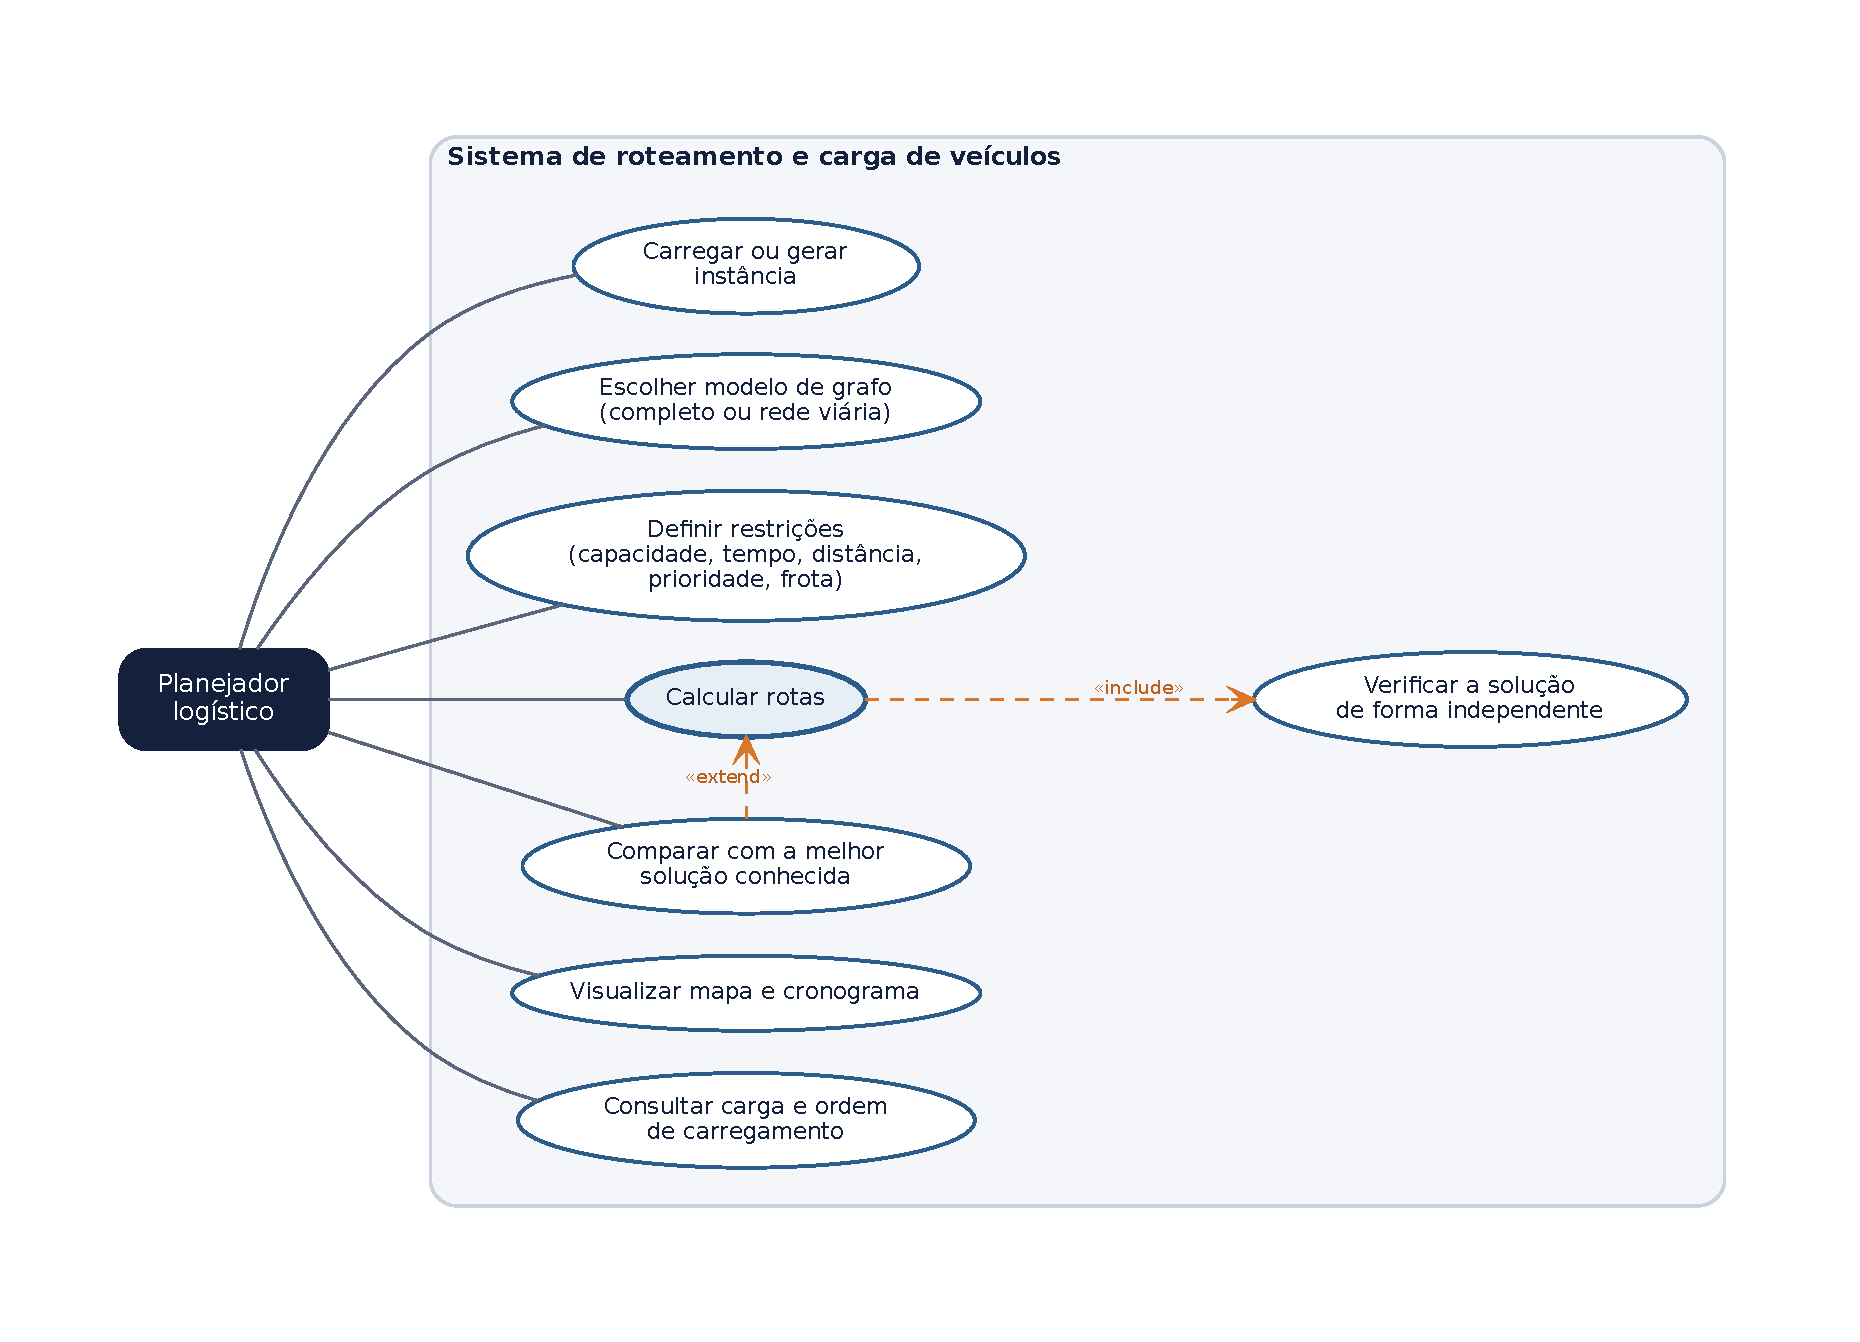
\includegraphics[width=\linewidth]{../diagramas/casos_de_uso.pdf}
\caption{Diagrama de casos de uso.}
\label{fig:casos}
\end{figure}

\begin{figure}[ht]
\centering
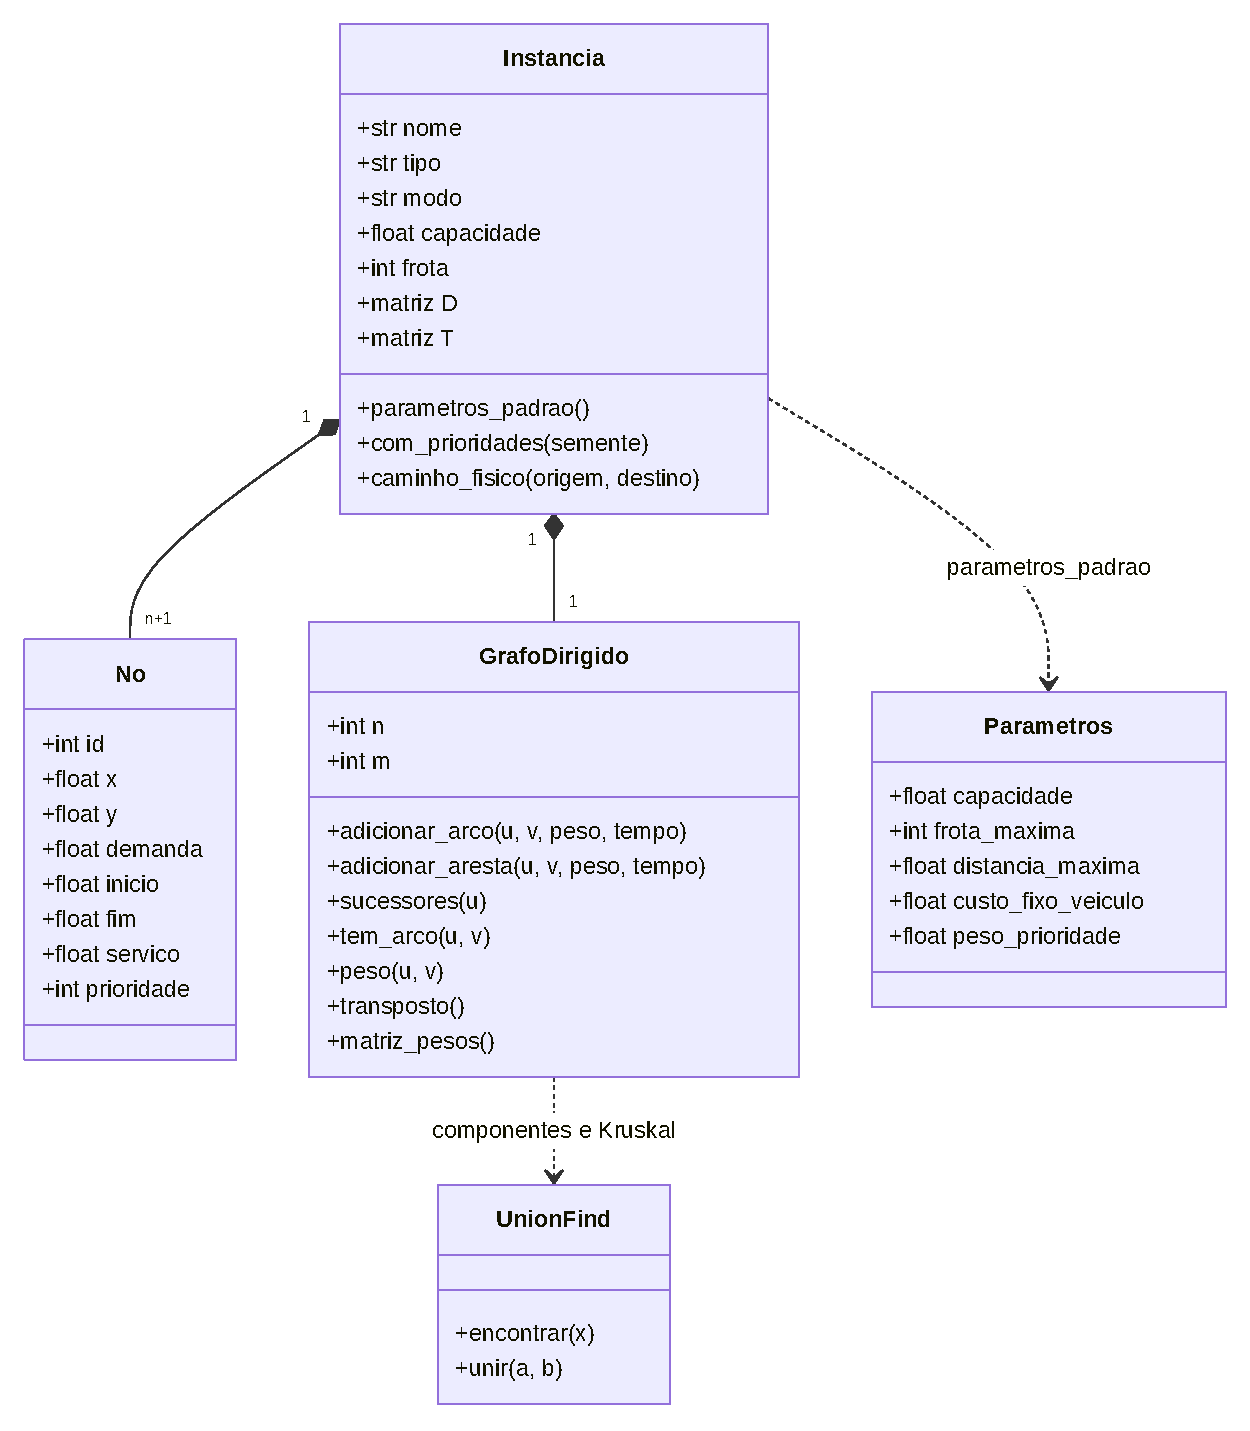
\includegraphics[width=0.66\linewidth]{../diagramas/classes_modelo.pdf}\\[4pt]
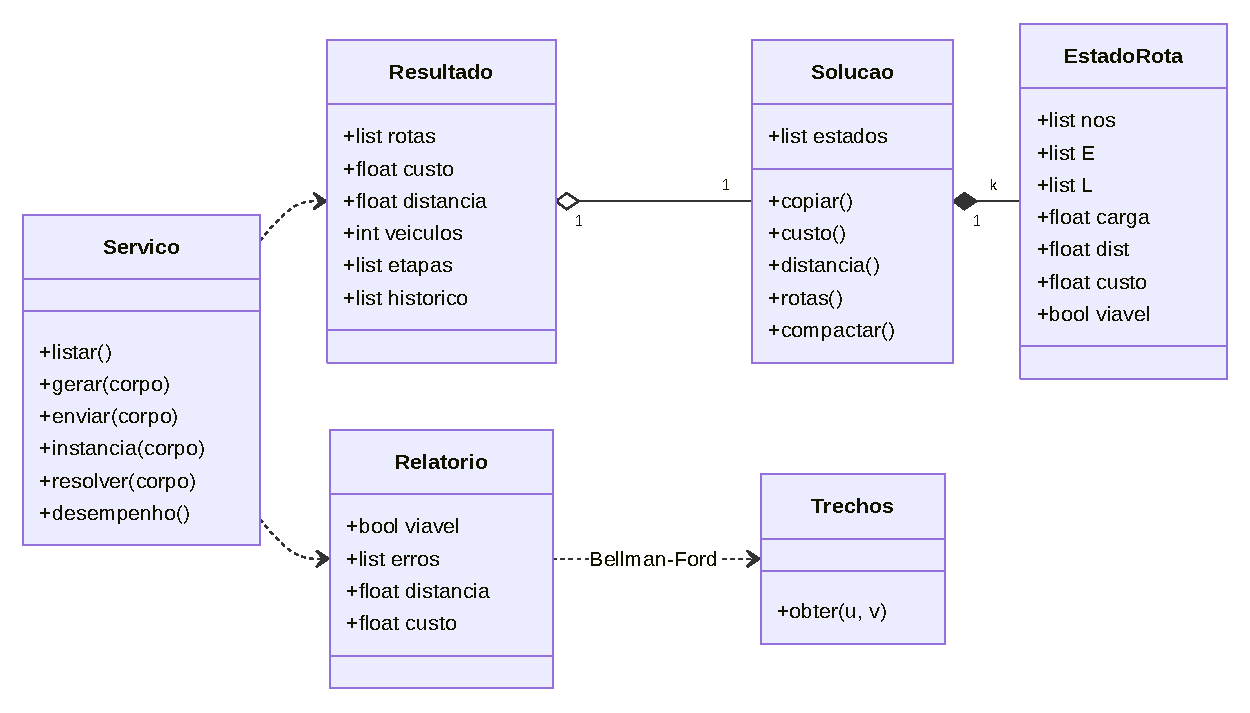
\includegraphics[width=\linewidth]{../diagramas/classes_execucao.pdf}
\caption{Diagramas de classes: modelo e grafo (acima) e solução, resultado e verificação (abaixo). Os algoritmos são funções de módulo.}
\label{fig:classes}
\end{figure}

\begin{figure}[ht]
\centering
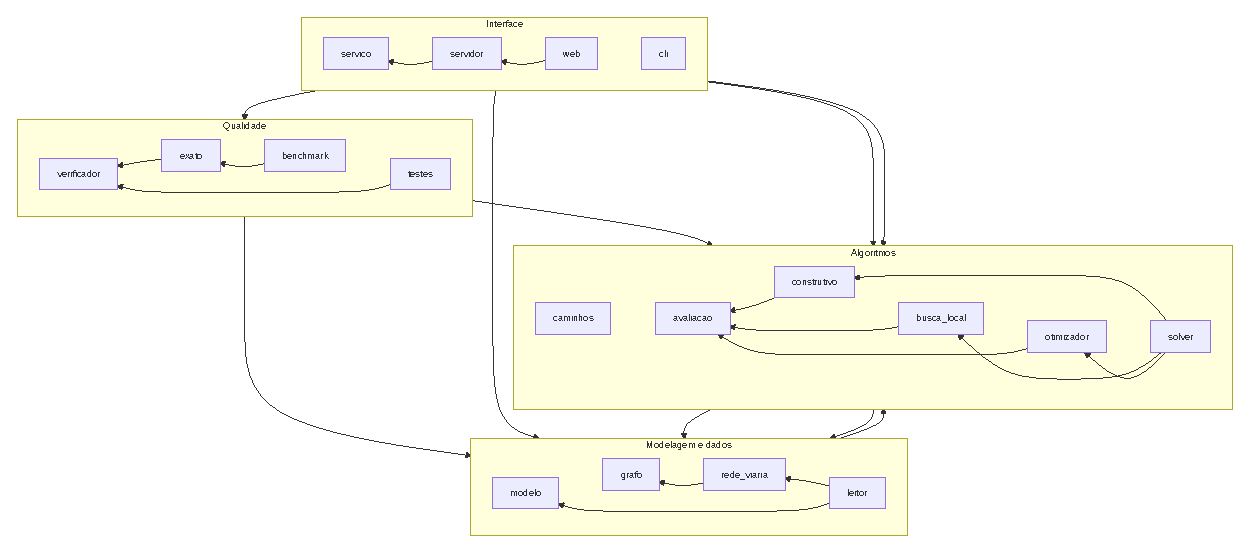
\includegraphics[width=\linewidth]{../diagramas/componentes.pdf}
\caption{Diagrama de componentes, agrupado pelas quatro frentes técnicas.}
\label{fig:comp}
\end{figure}

\begin{figure}[ht]
\centering
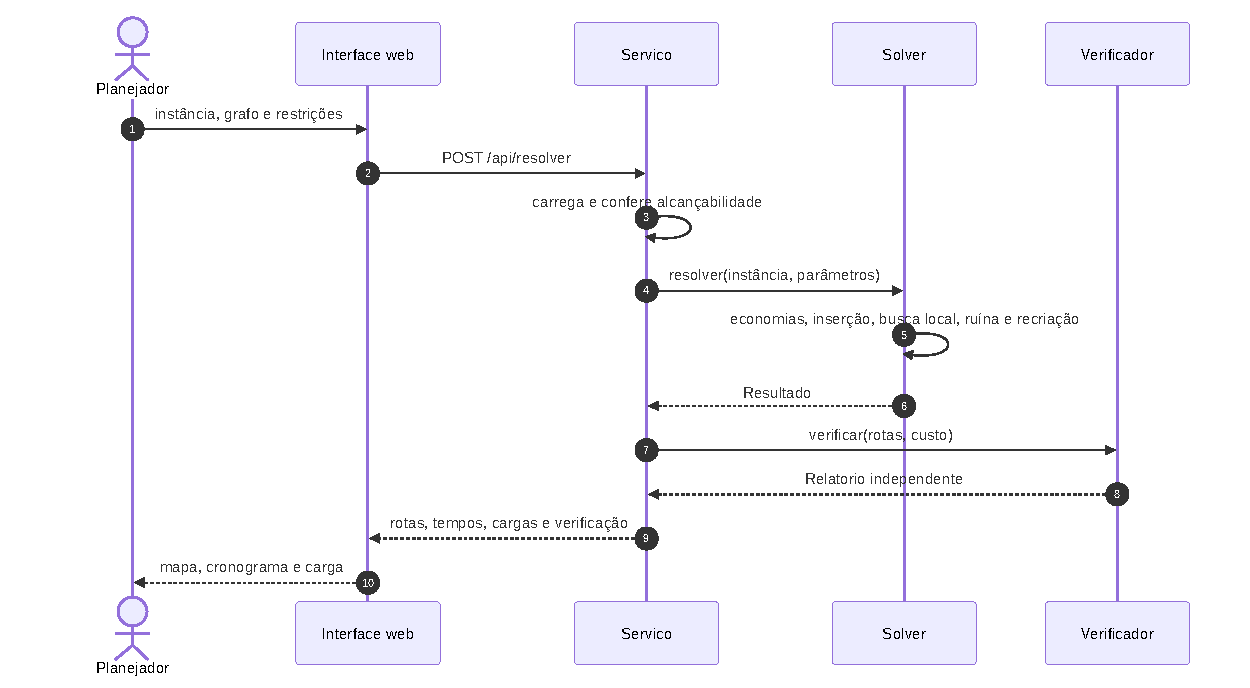
\includegraphics[width=\linewidth]{../diagramas/sequencia.pdf}
\caption{Diagrama de sequência da solicitação de cálculo de rotas.}
\label{fig:seq}
\end{figure}

\begin{figure}[p]
\centering
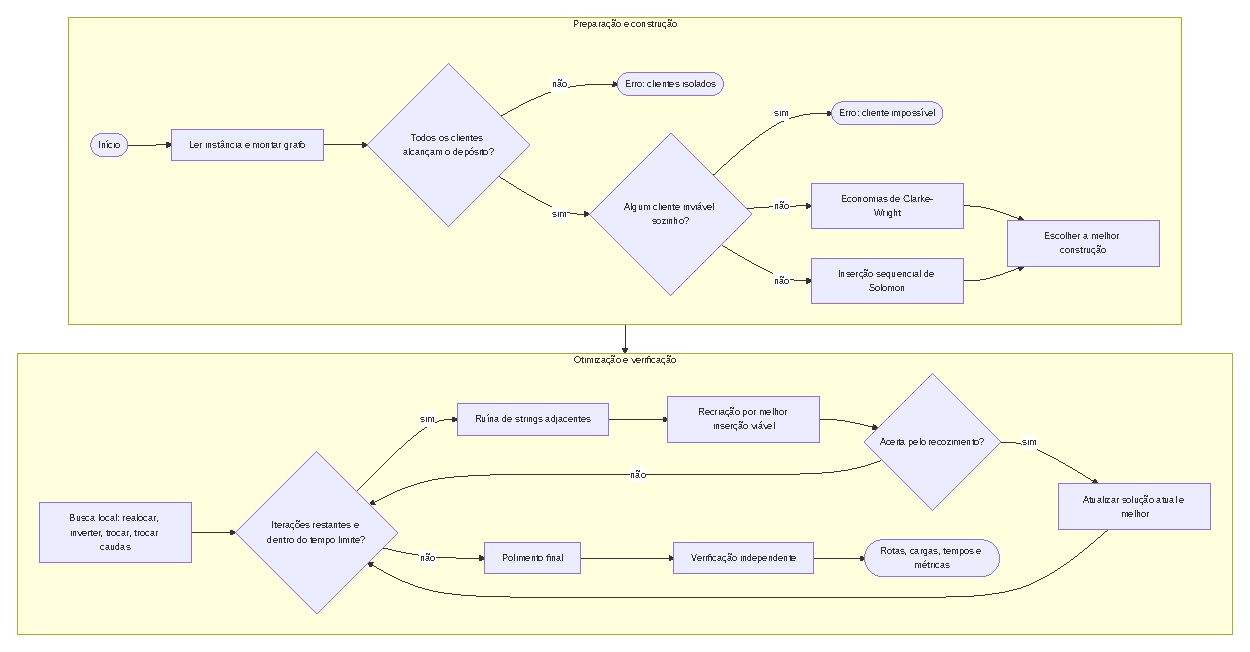
\includegraphics[width=\linewidth]{../diagramas/atividades.pdf}
\caption{Diagrama de atividades do solver.}
\label{fig:ativ}
\end{figure}

\section{Algoritmos escolhidos}

\begin{table}[!ht]
\centering
\small
\begin{tabular}{L{3.1cm}L{4.4cm}L{2.9cm}}
\toprule
Algoritmo & Papel na solução & Complexidade \\
\midrule
Dijkstra com heap \cite{dijkstra1959} & Custos e trajetos físicos no modo viário & $O((n+m)\log n)$ por origem \\
Kruskal com union-find \cite{kruskal1956} & Conexidade da rede viária & $O(m\log m)$ \\
BFS no grafo e no transposto & Detectar clientes inalcançáveis & $O(n+m)$ \\
Economias de Clarke-Wright \cite{clarke1964} & Solução inicial & $O(n^2\log n)$ \\
Inserção de Solomon \cite{solomon1987} & Solução inicial com janelas & $O(n^3)$ no pior caso \\
Folgas de tempo \cite{savelsbergh1985} & Testar inserção viável em tempo constante & $O(1)$ por posição \\
Busca local & Realocar, inverter, trocar, trocar caudas & polinomial por passo \\
Ruína e recriação \cite{christiaens2020} com recozimento \cite{kirkpatrick1983} & Melhoria da solução & $O(n)$ por iteração, em média \\
Bellman-Ford \cite{clrs2009} & Verificação independente dos custos viários & $O(nm)$ por origem \\
Enumeração exata & Referência em instâncias de até 8 clientes & $O(n\cdot n! + 3^n)$ \\
\bottomrule
\end{tabular}
\caption{Algoritmos, papel e complexidade.}
\end{table}

As escolhas seguem os requisitos do problema. Dijkstra serve porque os pesos são não negativos, e ele é mais rápido que Floyd-Warshall ($O(n^3)$) em grafos esparsos. Economias e inserção de Solomon geram pontos de partida diferentes, e o solver usa o melhor. A ruína e recriação foi escolhida por tratar bem restrições de tempo e capacidade sem penalidades: toda solução intermediária é viável. Métodos exatos de ramificação e preço não cabem no escopo da disciplina. Bibliotecas prontas de grafos \textbf{não} são usadas: estrutura, algoritmos e verificação são implementados pelo grupo, apenas com a biblioteca padrão do Python.

\section{Arquitetura}

O código está em Python 3 e usa só a biblioteca padrão. O pacote \texttt{logistica} é dividido em modelagem e dados, algoritmos, interface e qualidade (Figura~\ref{fig:comp}). A interface gráfica é uma página web servida localmente, com mapa, cronograma, carga por veículo e convergência. Os comentários no código são curtos e explicam só os pontos não óbvios; os nomes de módulos, funções e testes documentam o resto. Sem dependências externas, a ferramenta roda em qualquer máquina com Python, e a ausência de bibliotecas de grafos é deliberada: todas as estruturas e algoritmos foram escritos para este trabalho.

\section{Plano de desenvolvimento}

\subsection{Fases e marcos}

\begin{table}[!ht]
\centering
\small
\begin{tabular}{L{2.2cm}L{8.4cm}}
\toprule
Marco & Entregas \\
\midrule
Até 12/11 & Etapa 1: este documento, modelagem, UML e matriz de requisitos \\
Até 17/11 & Etapa 2: grafo, algoritmos, interface, testes e repositório Git \\
Até 20/11 & Etapa 3: experimentos, relatório em LaTeX (SBC), vídeo e slides \\
22/11 & Entrega de cada integrante no Canvas até as 23:59 \\
\bottomrule
\end{tabular}
\caption{Cronograma.}
\end{table}

\subsection{Divisão de responsabilidades}

Cada integrante desenvolve sua parte em uma branch própria, e as branches são integradas à branch principal com merge commit, preservando o histórico de cada um. Essa divisão deixa claro quem responde por qual parte e permite que cada integrante explique suas funcionalidades na apresentação, sem perder a visão do conjunto. O diagrama de casos de uso e a estrutura e o estilo da interface eram, no início, de outro integrante, que deixou a disciplina durante a Etapa~3. Essas partes foram refeitas por João Gabriel, com um visual novo e o mesmo conteúdo.

\begin{table}[!ht]
\centering
\small
\begin{tabular}{L{2.2cm}L{8.4cm}}
\toprule
Integrante & Responsabilidades \\
\midrule
João Gabriel & Estrutura inicial do repositório, integração das branches na principal e commits de ajuste (arquivos fora do lugar, arquivo que faltava, READMEs de cada pasta); modelo e grafo dirigido (union-find, Kruskal, alcançabilidade); leitura das bases (VRPLIB, texto de Solomon e CSV do Kaggle) e rede viária; serviço, servidor HTTP e interface web (estrutura, estilo e lógica: mapa, cronograma, carga, convergência); diagrama de casos de uso e diagramas de classes; experimentos, figuras e tabelas; documento da Etapa 1 e relatório final \\
Pedro Eduardo & Levantamento das bases de dados; diagramas de componentes e de sequência; avaliação de rotas com folgas de tempo; heurísticas construtivas; busca local com filtros $O(1)$; ruína e recriação e solver; verificador independente; solver exato; testes com os dados do Kaggle \\
Thomas Ramos & Diagrama de atividades; caminhos mínimos com Dijkstra e seus testes; linha de comando; tutorial de uso \\
\bottomrule
\end{tabular}
\caption{Divisão das responsabilidades.}
\end{table}

\subsection{Estratégia de testes e critérios de aceitação}

\begin{itemize}
  \item Dijkstra contra Floyd-Warshall e Kruskal contra enumeração de árvores, em grafos aleatórios, com pesos iguais, zeros e grafos desconexos.
  \item Inserção em tempo constante contra recálculo completo da rota.
  \item Reprodução do custo das 65 BKS por um verificador independente, que recalcula distâncias das coordenadas e usa Bellman-Ford.
  \item Comparação com o solver exato em instâncias pequenas, e comparação com as BKS nas grandes.
  \item Entradas inválidas na leitura e na API: arquivo ausente, capacidade menor que a demanda, rede desconexa, cliente impossível.
  \item Aceitação: toda solução exibida passa pela verificação independente, e o resultado é reproduzível por semente.
\end{itemize}

\subsection{Riscos}

\begin{description}
  \item[Heurística sem garantia de otimalidade:] mitigada pela comparação com BKS e solver exato; a diferença é sempre reportada.
  \item[Desempenho de Python:] limitamos o tamanho dos experimentos e medimos o tempo por fase.
  \item[Dados sintéticos de prioridade e rede viária:] declarados como tais; as conclusões sobre eles não são generalizadas.
  \item[Prazo:] todas as etapas têm a mesma data de entrega; os marcos acima antecipam a revisão.
\end{description}

\bibliographystyle{sbc}
\bibliography{../../relatorio/referencias}
\end{document}
